\section{引言}

\subsection{\TeX{} 与 \LaTeX}

\begin{frame}[fragile]{\TeX{} 与 \LaTeX}
  \begin{columns}[T]
    \column{.8\textwidth}
    \begin{itemize}
      \item \TeX{}
            \begin{itemize}
              \item 生成精美图书的排版系统
              \item 最初由 Donald Knuth(高德纳)于 1978 年开发
              \item 每 7 年发布新版,最新版本为 \TeX{} 3.141592653(2021 年 1 月)\link{https://tex.stackexchange.com/questions/581118/whats-new-in-tex-version-3-141592653}
              \item 漂亮、美观、稳定、通用
              \item 尤其擅长数学公式排版
            \end{itemize}
      \item \LaTeX{}
            \begin{itemize}
              \item Leslie Lamport 开发的一种 \TeX{} 格式
              \item 原版 \TeX{} 过于晦涩难懂,\CJKsout{不适合正常人类}
              \item 在 \TeX{} 的基础上提供更多命令,降低使用门槛
              \item 极其丰富的宏包,提供扩展功能
              \item 广泛用于学术界,有各种论文模板
                    % \item 大学学位论文模板,如 \hithesis
            \end{itemize}
    \end{itemize}
    \column{.2\textwidth}
    \vspace*{5mm}
    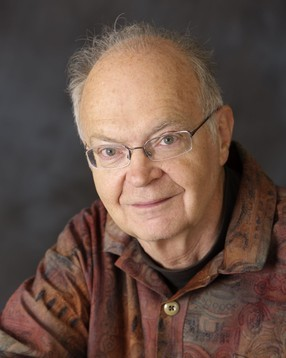
\includegraphics[width=\textwidth]{Knuth.jpg}

    \vspace*{5mm}
    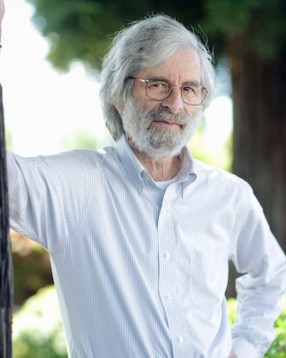
\includegraphics[width=\textwidth]{Lamport.jpg}

  \end{columns}
\end{frame}

\begin{frame}[fragile]{没什么用的知识}
  \begin{itemize}
    \item 关于名字
          \begin{itemize}
            \item \TeX{} 这个名字来源于希腊语词根 τεχ--
            \item \LaTeX{} 则比较简单粗暴:La 就是 Lamport 的意思
          \end{itemize}
    \item 关于读音
          \begin{itemize}
            \item Knuth 坚持要求将 \TeX{} 读作 \textipa{/tEx/},类似“泰赫”
            \item 不过 Lamport 认为 \LaTeX{} 的读音无所谓
          \end{itemize}
    \item 关于拼写
          \begin{itemize}
            \item \TeX{} 一般都会拼成这样错落有致的样子,主要是为了:
                  \begin{itemize}
                    \item 通过奇奇怪怪的排版效果,说明这是一个排版系统的名字
                    \item 与其他名字区分开,比如当年还有一个叫 TEX 的系统
                  \end{itemize}
            \item 如果环境不支持这种排版,则应该拼写为 TeX
            \item 后来 \TeX{} 的衍生产品往往都有类似的做法
                  \begin{itemize}
                    \item \LaTeX{}、\BibTeX{}、\XeTeX{}、\CTeX{}……
                  \end{itemize}
          \end{itemize}
  \end{itemize}
\end{frame}

% \begin{frame}{和 Word 对比}
%   注:术业有专攻,评价需客观
%   \begin{table}[h]
%     \centering
%     % \rowcolors[]{1}{primaryL}{primaryL!40}
%     \begin{tabular}{c|c}
%       Microsoft\textsuperscript{\textregistered}  Word & \LaTeX{}        \\
%       \hline
%       字处理工具                                            & 专业排版软件        \\
%       容易上手,简单直观                                        & 容易上手          \\
%       所见即所得                                            & 所见即所想,所想即所得   \\
%       高级功能不易掌握                                         & 进阶难,但一般用不到    \\
%       处理长文档需要丰富经验                                      & 和短文档处理基本无异    \\
%       花费大量时间调格式                                        & 无需担心格式,专心作者内容 \\
%       公式排版差强人意                                         & 尤其擅长公式排版      \\
%       二进制格式,兼容性差                                       & 文本文件,易读、稳定    \\
%       付费商业许可                                           & 自由免费使用        \\
%     \end{tabular}
%   \end{table}
% \end{frame}

\subsection{\LaTeX{} 排版展示}

\begin{frame}[fragile]{\LaTeX{} 用起来究竟什么样?}
  \vspace{1em}
  \begin{columns}
    \begin{column}{0.55\textwidth}
      \begin{texcode}[gobble=8,basicstyle=\tiny\ttfamily, moretexcs={\maketitle},emph={[1]equation,itemize,document}, emph={[2]article,amsmath,graphicx}]
        \documentclass{article}
        \usepackage{amsmath,graphicx}
        \title{Normal distribution}
        \author{Wikipedia, the free encyclopedia}

        \begin{document}
          \maketitle
          \section{Introduction}
          % 省略一些内容……
          The probability density of the normal
          distribution is
          \begin{equation}
            f(x|\mu, \sigma)
            = \frac{1}{\sqrt{2\pi\sigma^2}}
            e^{-\frac{(x-\mu)^2}{2\sigma^2}}
          \end{equation}
          where
          \begin{itemize}
            \item $\mu$ is the mean of the distribution
            \item $\sigma$ is the standard deviation
          \end{itemize}
        \end{document}
      \end{texcode}
    \end{column}

    \begin{column}{0.45\textwidth}
      \begin{figure}
        \centering
        \vspace{-0.8cm}
        \includegraphics[width=\textwidth, trim={2cm 2cm 2cm 2cm}, clip]%
        {examples/normal-dist/normal-dist.pdf}
      \end{figure}
    \end{column}
  \end{columns}
  % \nonumberfootnote{来源:Wikipedia \link{https://en.wikipedia.org/wiki/Normal_distribution}}
\end{frame}

% \begin{frame}{基本原则}
%   \begin{itemize}
%     \item 排版 vs 文字处理
%           \begin{itemize}
%             \item 《别把 \LaTeX{} 当 Word 用》
%           \end{itemize}
%     \item 遵循业(xué)界(xiào)规范
%           \begin{itemize}
%             \item 《管教务处 or 研究生院 or 物理系叫爸爸》
%           \end{itemize}
%           % \item 追求良好的阅读体验\zhparen{readability}
%     \item 内容与格式分离
%     \item \alert{内容永远比格式重要!}
%           \begin{itemize}
%             \item \emph{Typography exists to honor content.} ---R. Bringhurst
%           \end{itemize}
%   \end{itemize}
% \end{frame}

\begin{frame}{\LaTeX{} 排版展示:文本}
  \vspace{1em}
  \begin{columns}
    \begin{column}{.45\textwidth}
      \begin{figure}
        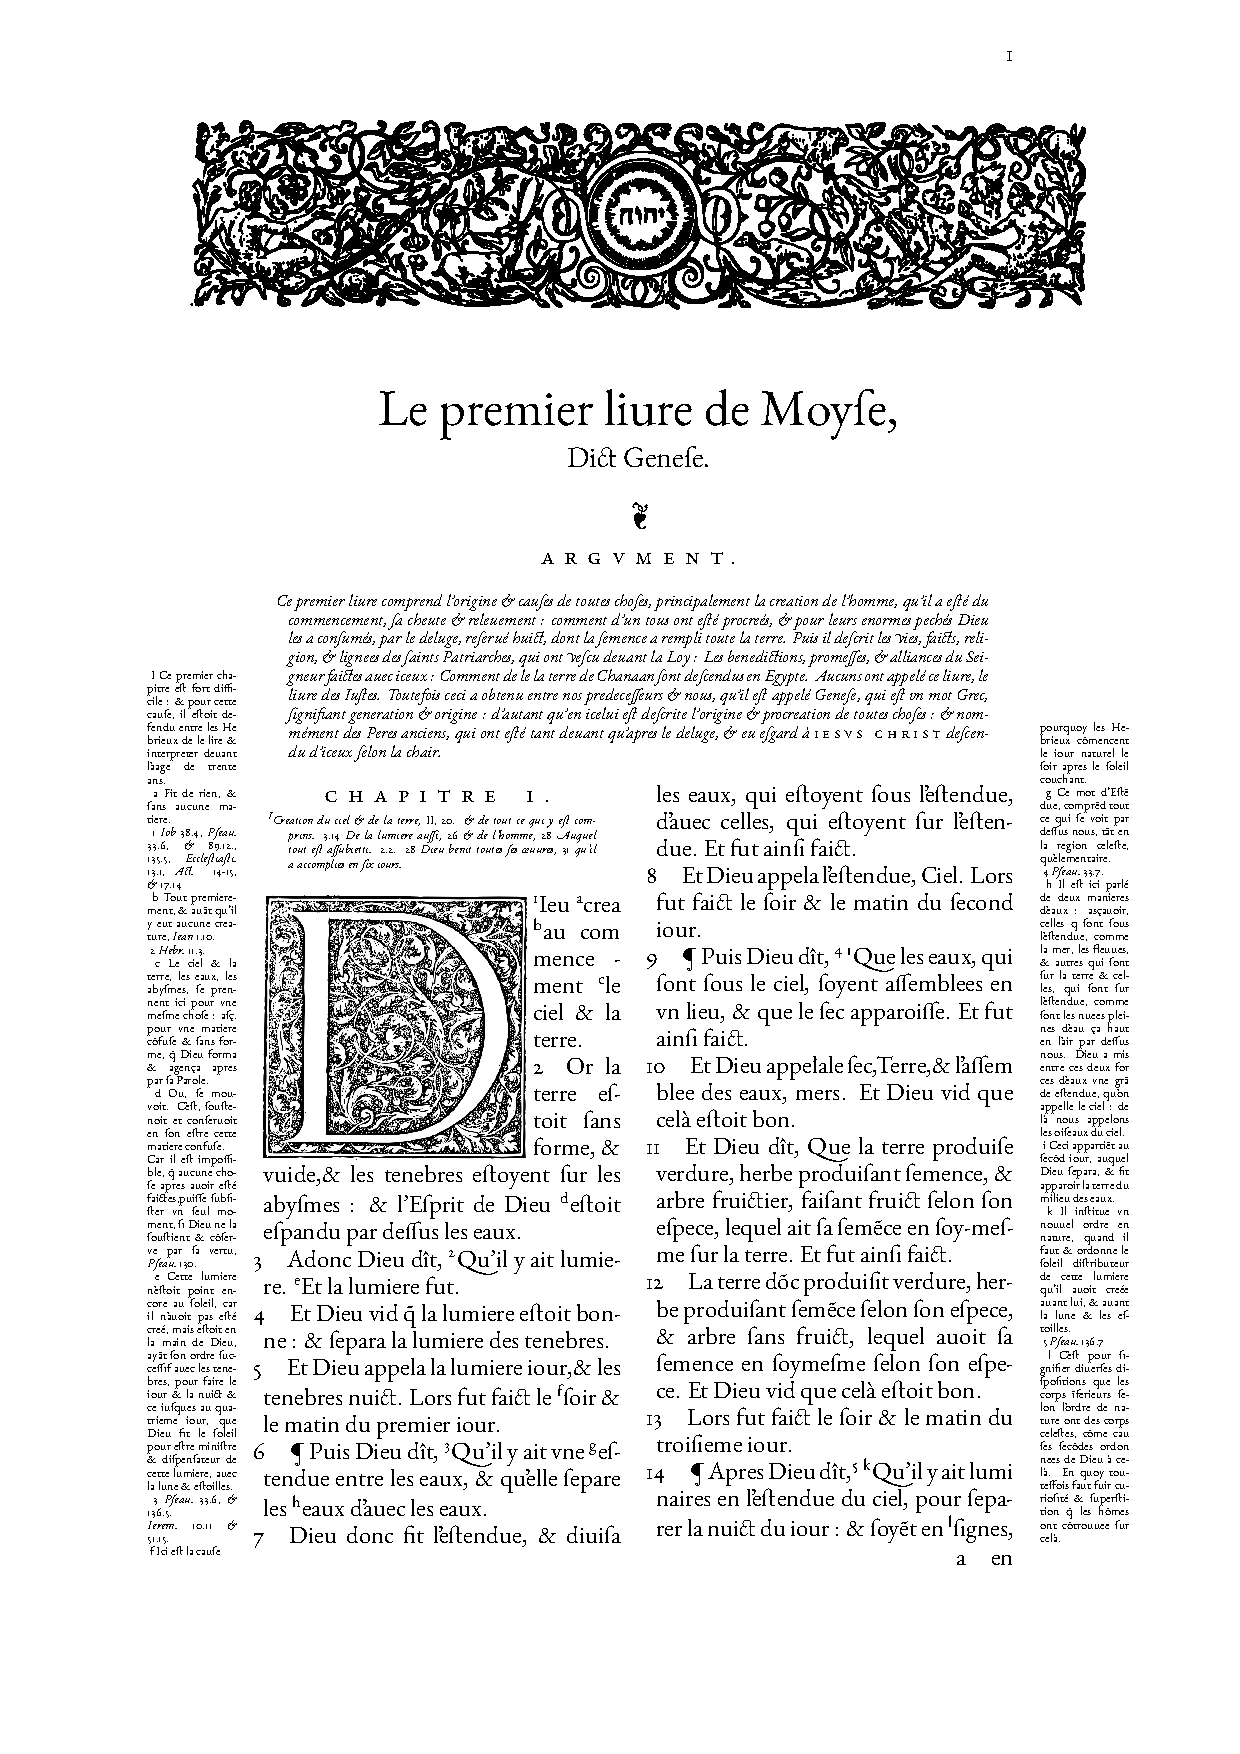
\includegraphics[width=\textwidth,page=1]{geneve_1564.pdf}
      \end{figure}
    \end{column}
    \begin{column}{.45\textwidth}
      \begin{figure}
        \includegraphics[width=\textwidth,page=2]{geneve_1564.pdf}
      \end{figure}
    \end{column}
  \end{columns}
\end{frame}

\begin{frame}{\LaTeX{} 排版展示:公式}
  \begin{align*}
    \oiint_{\partial\Omega} \V{E} \cdot \dd \V{S}
     & = \frac{1}{\epsilon_0} \iiint_\Omega \rho \, \dd V      \\
    \oiint_{\partial\Omega} \V{B} \cdot \dd \V{S}
     & = 0                                                     \\
    \oint_{\partial\Sigma} \V{E} \cdot \dd \V{l}
     & = -\frac{\dd}{\dd t} \iint_\Sigma \V{B} \cdot \dd \V{S} \\
    \oint_{\partial\Sigma} \V{B} \cdot \dd \V{l}
     & = \mu_0 \left( \iint_\Sigma \V{J} \cdot \V{S}
    + \epsilon_0 \frac{\dd}{\dd t} \iint_\Sigma \V{E} \cdot \dd \V{S} \right)
  \end{align*}
\end{frame}

\begin{frame}{\LaTeX{} 排版展示:图形}
  \begin{figure}
    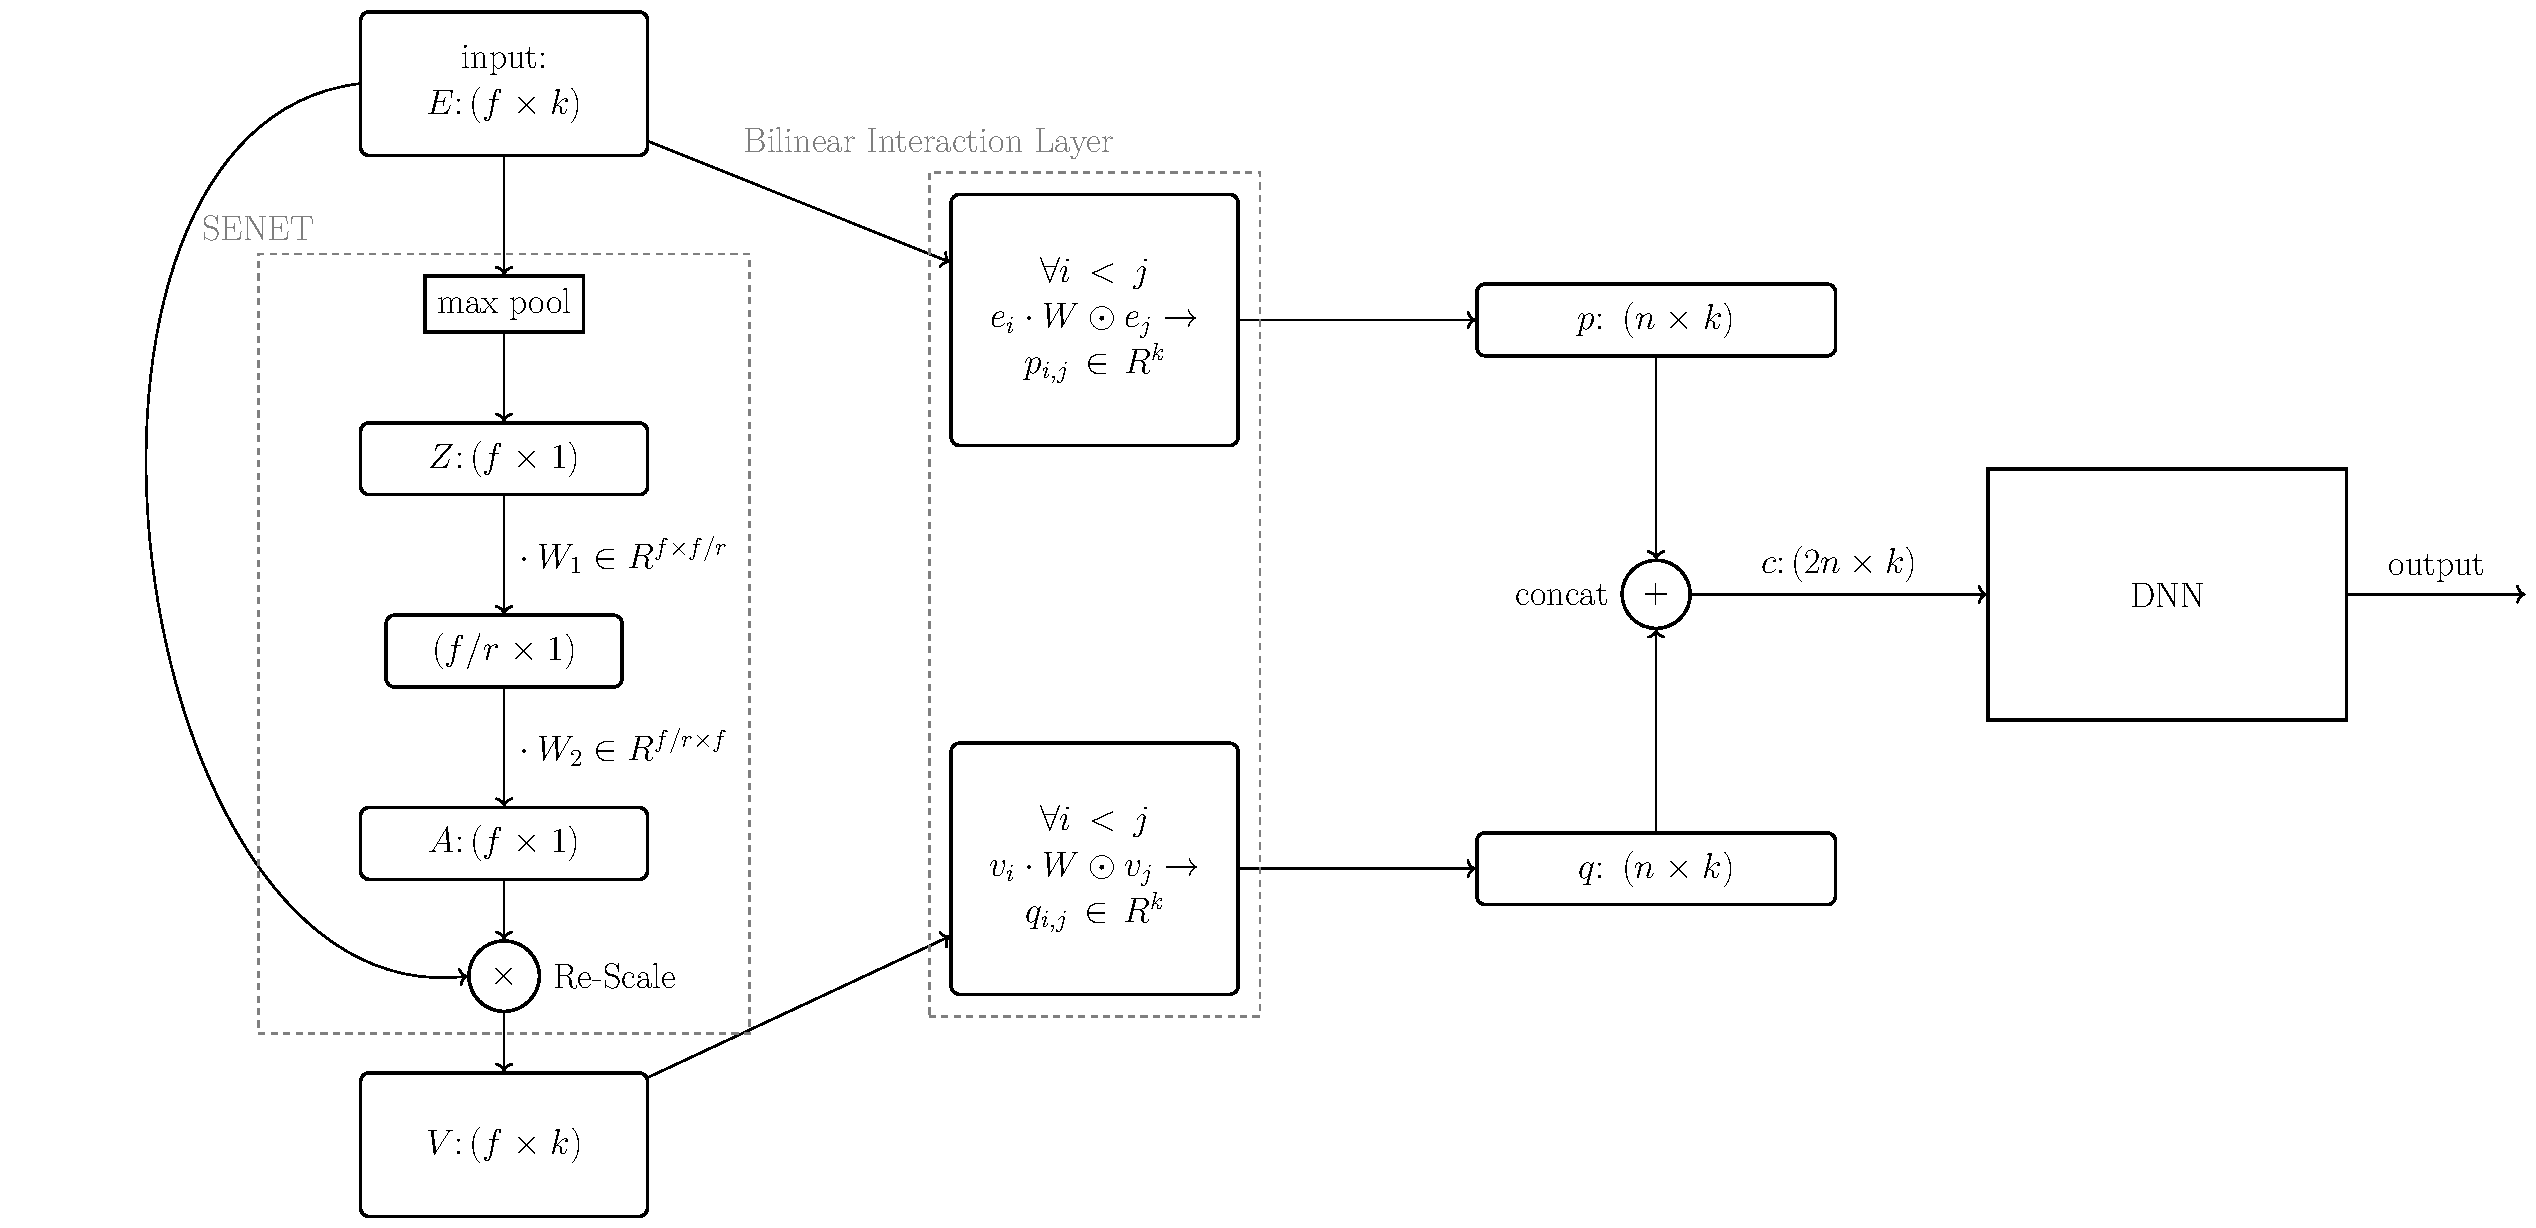
\includegraphics[width=\textwidth]{flowchart.pdf}
  \end{figure}
\end{frame}

\begin{frame}{\LaTeX{} 排版展示:幻灯片}
  \begin{columns}
    \begin{column}{.5\textwidth}
      \begin{figure}
        
\includegraphics[width=\textwidth]{slides_xiaoshan.pdf}
      \end{figure}
    \end{column}
    \begin{column}{.5\textwidth}
      \begin{figure}
        
\includegraphics[width=\textwidth]{slides_hit.pdf}
      \end{figure}
    \end{column}
  \end{columns}
\end{frame}

\begin{frame}{\LaTeX{} 排版展示:简历}
  \vspace{1em}
  \begin{columns}
    \begin{column}{.45\textwidth}
      \begin{figure}
        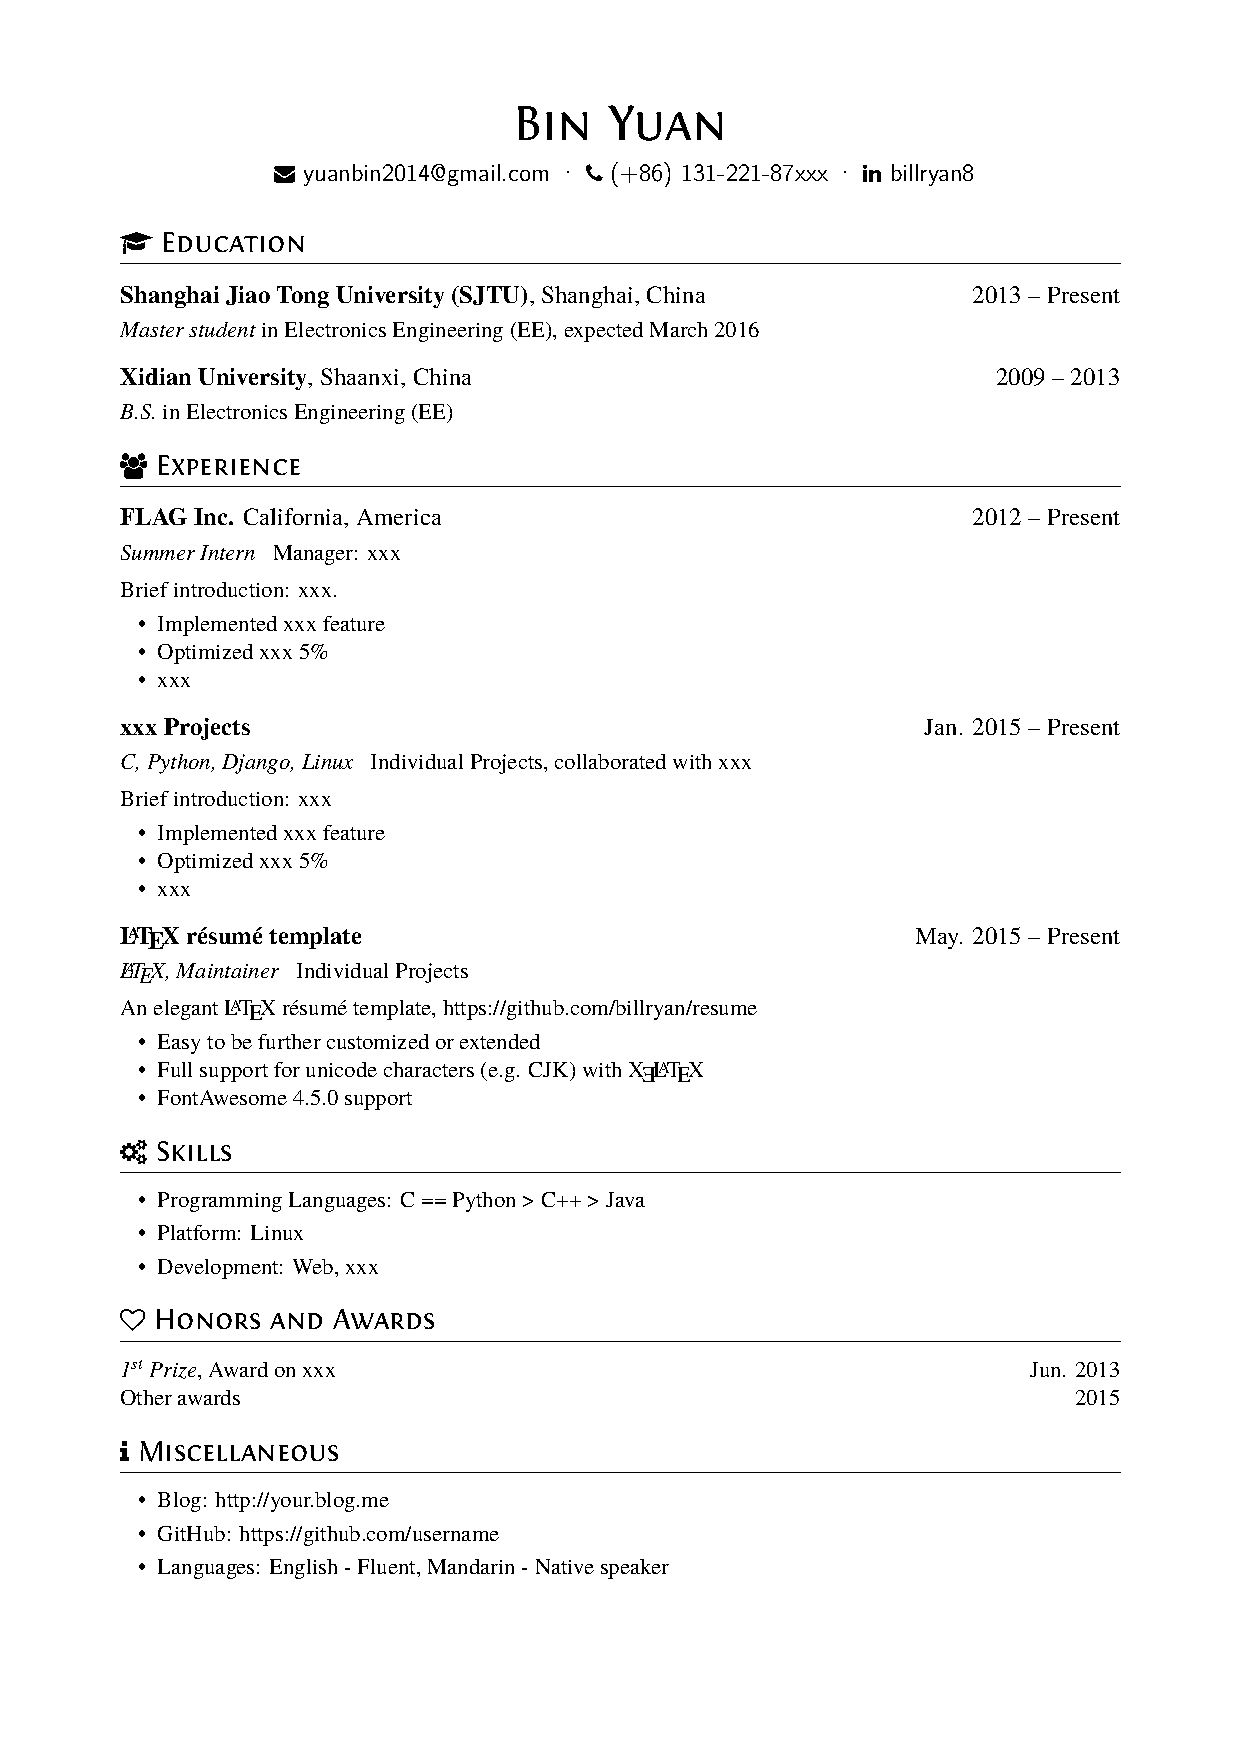
\includegraphics[width=\textwidth]{resume.pdf}
      \end{figure}
    \end{column}
    \begin{column}{.45\textwidth}
      \begin{figure}
        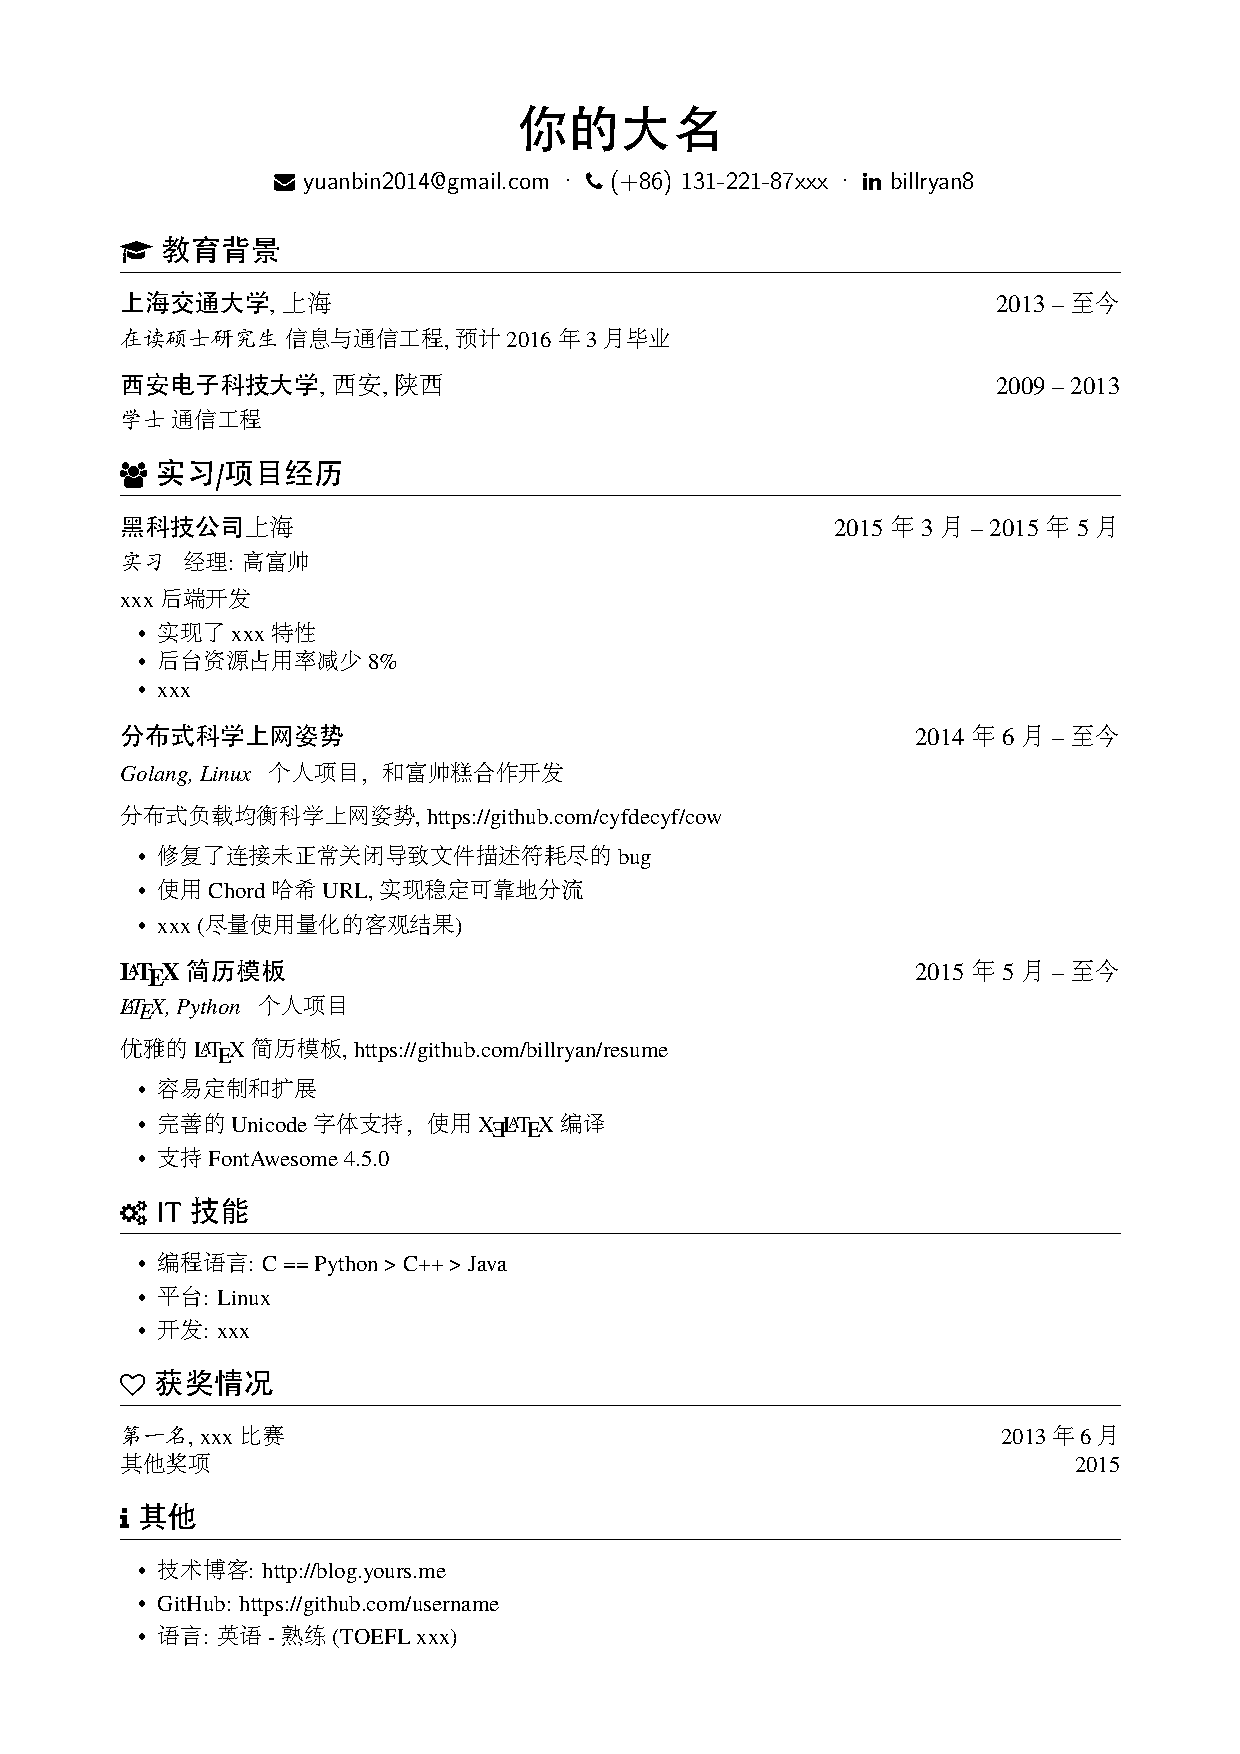
\includegraphics[width=\textwidth]{resume-zh_CN.pdf}
      \end{figure}
    \end{column}
  \end{columns}
\end{frame}

% \begin{frame}{\LaTeX{} 排版示例:公式}
%   \begin{align*}
%     \oiint_{\partial\Omega} \V{E} \cdot \dd \V{S}
%      & = \frac{1}{\epsilon_0} \iiint_\Omega \rho \, \dd V
%      & \quad                                              &
%     \oint_{\partial\Sigma} \V{E} \cdot \dd \V{l}
%     = -\frac{\dd}{\dd t} \iint_\Sigma \V{B} \cdot \dd \V{S} \\
%     \oiint_{\partial\Omega} \V{B} \cdot \dd \V{S}
%      & = 0
%      & \quad                                              &
%     \oint_{\partial\Sigma} \V{B} \cdot \dd \V{l}
%     = \mu_0 \iint_\Sigma \V{J} \cdot \V{S}
%     + \mu_0 \epsilon_0 \frac{\dd}{\dd t} \iint_\Sigma \V{E} \cdot \dd \V{S}
%   \end{align*}
% \end{frame}
